\documentclass{article}
\usepackage{hyperref}
\usepackage[margin=0.5in]{geometry}
\usepackage{amsmath}
\usepackage{graphicx}
\graphicspath{ {./assets/} }

\title{PHYSIOL 578: HW1\footnotetext{U-M GPT was used to refine language of answers derived independently.}}
\author{Jack Yang \\ \href{mailto:yhyunjoo@umich.edu}{yhyunjoo@umich.edu}}
\date{September 4, 2026}

\begin{document}
\maketitle
\section{Describe a physiologic homeostatic system. Do not use an example from class. If you work with others, your answer should be unique (each student should choose a unique homeostatic system). A drawing may be very helpful. Identify the key components of the homeostatic system and describe briefly how they function and interact. Use a single page for your response.}
In blood glucose homeostasis, pancreatic alpha and beta cells monitor glucose levels in the bloodstream. If glucose levels are too high, pancreatic beta cells release the hormone insulin, which signals skeletal muscle fibers and fat cells to take up glucose and promotes glucose storage in liver cells. These responses lower the concentration of glucose in the bloodstream.

Conversely, if blood glucose levels fall too low, beta cells reduce insulin release, and alpha cells are stimulated to release glucagon. Glucagon raises blood glucose by signaling the liver to perform glycogenolysis and gluconeogenesis.
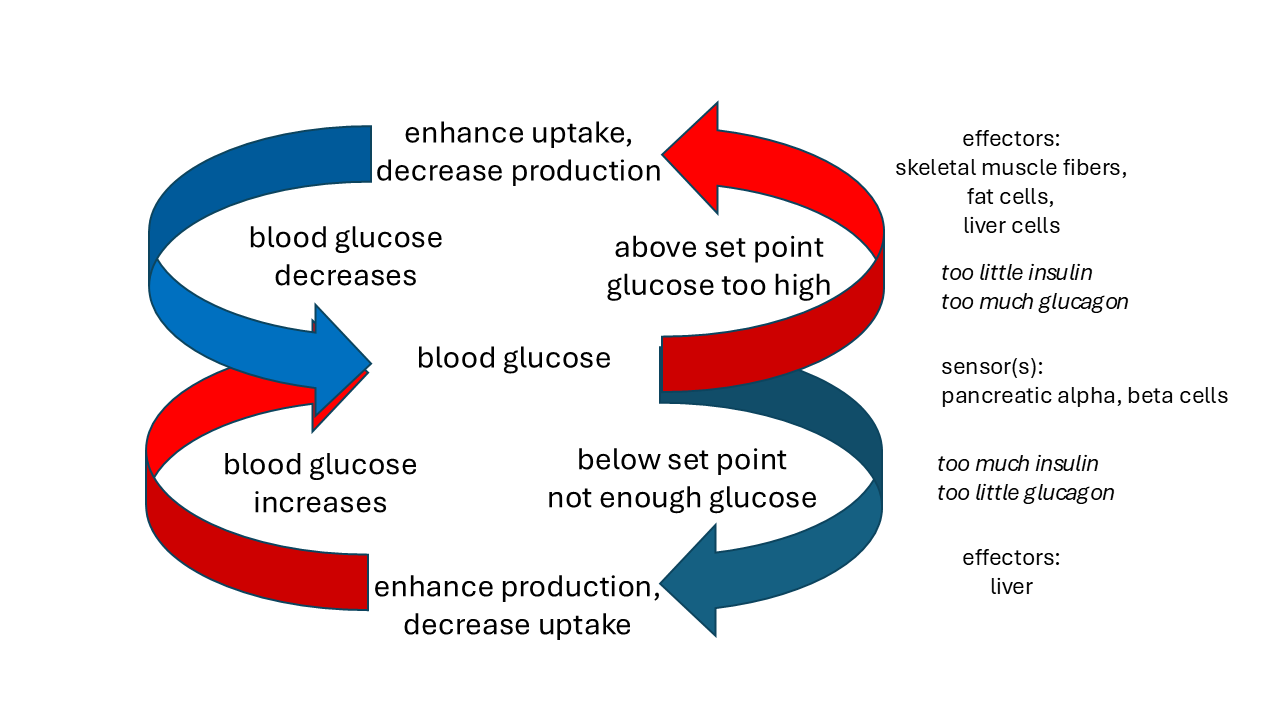
\includegraphics[width=\textwidth]{fig1}

\newpage
\section{Check the hummingbird folder in this section. Explain how a hummingbird can fly across the Gulf of Mexico.}

Hummingbirds have extremely high metabolic demands during flight and therefore feed frequently.
Before migration, they consume excess nectar and convert surplus carbohydrates into fat, building substantial energy reserves.
During normal feeding, they can fuel flight largely through the direct oxidation of dietary sugars.
During the long, nonstop flight across the Gulf of Mexico, however, they rapidly switch to oxidizing stored fatty acids.
Because fat stores much more energy per unit mass than carbohydrates, this metabolic flexibility and high capacity for fatty-acid oxidation allow hummingbirds to sustain the journey.

\section{Ohm's Law: explain how ion channels affect input resistance.}
In a cell, ionic current is given by
$$I = g(V-E_{\text{rev}})$$
where: \\
$I$ is the ionic current \\
$g$ is conductance (inverse of resistance $1/R$) \\
$V-E_{\text{rev}}$ is the driving potential
\\

The driving potential $V-E_{\text{rev}}$ is generated by the electrochemical gradient across the membrane.
Because the membrane is relatively impermeable to ions, the resistance $R$ is very high (conductance $g$ is low) and there is hardly any ions crossing the membrane, thus minimal ionic current $I$, even when there is a driving potential.
However, with ion channels that allow ions to pass through the membrane according to the driving potential, the current $I$ increases and \textbf{resistance $R$ decreases}.


\section{ The Nernst Equation: calculate the reversal potential for a channel permeable to a single ion. Name the ion and the concentrations you chose and why you chose them (``because I found them in a book'' is not a good answer). Be sure to list all parameters.}
Nernst Equation is given by
$$E_{\text{rev}} = \frac{RT}{zF}\ln\frac{[\text{Ion}]_{\text{out}}}{[\text{Ion}]_{\text{in}}}$$
where: \\
$R$ is the universal ideal gas constant \\
$T$ is temperature in kelvins \\
$z$ is the charge \\
$F$ is Faraday's constant \\
$[\text{Ion}]$ is the concentration of the ion
\\

Kir2.1 is an inward-rectifier potassium channel that is permeable mostly to K\textsuperscript{+}. Thus its reversal potential $E_\text{rev}$ can be calculated by:

$$E_{\text{rev}} = \frac{RT}{(1)F}\ln\frac{4\times10^{-3}\text{M}}{1.35\times10^{-1}\text{M}}$$
$$= \frac{(8.314\text{J/(mol}\cdot\text{K)})(310.15\text{K})}{(1)(9.648\times10^4\text{C/mol})}(-3.519) = \frac{2.578\times10^{3}\text{J/mol}}{9.648\times10^4\text{C/mol}}(-3.519)$$
$$= -0.094\text{J/C} = \boxed{-94\text{mV}}$$
where: \\
$T = 310.15\text{K}$ as the temperature of the body \\
$z = +1$ as K\textsuperscript{+} has charge of +1 \\
$[\text{Ion}]_{\text{in}} = 1.35\times10^{-1}\text{M}$ as the normal intracellular concentration of K\textsuperscript{+} for a mammalian neuron \\
$[\text{Ion}]_{\text{out}} = 4\times10^{-3}\text{M}$ as the normal extracellular concentration of K\textsuperscript{+} for a mammalian neuron
\\

Therefore, for a Kir2.1 channel in a mammalian neuron with $135\text{mM}$ intracellular K\textsuperscript{+} and $4\text{mM}$ extracellular K\textsuperscript{+} at $37^{\circ}\text{C}$, the predicted reversal potential is $\boxed{-94\text{mV}}$.

\section{GHK equation: use physiologic concentrations appropriate for the squid giant axon. Estimate the resting potential of the axon. What might complicate your answer? Be sure to list all parameters you used in your calculation.}
The GHK equation is given by
$$E_\text{GHK} = \frac{RT}{F}\ln\frac{p_{\text{K}}[\text{K}]_{\text{out}}+p_{\text{Na}}[\text{Na}]_{\text{out}}+p_{\text{Cl}}[\text{Cl}]_{\text{in}}}{p_{\text{K}}[\text{K}]_{\text{in}}+p_{\text{Na}}[\text{Na}]_{\text{in}}+p_{\text{Cl}}[\text{Cl}]_{\text{out}}}$$
where: \\
$R$ is the universal ideal gas constant \\
$T$ is temperature in kelvins \\
$F$ is Faraday's constant \\
$[\text{Ion}]$ is the concentration of the ion \\
$p_{Ion}$ is the relative permeability of ion
\\

Then the resting potential of the squid giant axon can be estimated by:
$$E_{\text{GHK}} = \frac{(8.314\text{J/(mol}\cdot\text{K)})(298.15\text{K})}{9.648\times10^4\text{C/mol}}\ln\frac{(1)(20\text{mM}) + (0.04)(440\text{mM}) + (0.45)(40\text{mM})}{(1)(400\text{mM}) + (0.04)(50\text{mM}) + (0.45)(560\text{mM})}$$
$$= \frac{(8.314\text{J/(mol}\cdot\text{K)})(298.15\text{K})}{9.648\times10^4\text{C/mol}}(-2.465) = (25.69\text{mV})(-2.465)$$
$$= \boxed{-63.326\text{mV}}$$
where: \\
$T = 298.15K$ is the temperature within the functional range of squid physiology \\ 
$p_K = 1$ is the relative permeability of K\textsuperscript{+} \\
$p_\text{Na} = 0.04$ is the relative permeability of Na\textsuperscript{+} \\
$p_\text{Cl} = 0.45$ is the relative permeability of Cl\textsuperscript{-} \\
$[\text{K}]_{\text{out}} = 20\text{mM}$ is the concentration of extracellular potassium in squid giant axon \\
$[\text{K}]_{\text{in}} = 400\text{mM}$ is the concentration of intracellular potassium in squid giant axon \\
$[\text{Na}]_{\text{out}} = 440\text{mM}$ is the concentration of extracellular sodium in squid giant axon \\
$[\text{Na}]_{\text{in}} = 50\text{mM}$ is the concentration of intracellular sodium in squid giant axon \\
$[\text{Cl}]_{\text{out}} = 560\text{mM}$ is the concentration of extracellular chloride in squid giant axon \\
$[\text{Cl}]_{\text{in}} = 40\text{mM}$ is the concentration of intracellular chloride in squid giant axon \\
\\

The answer is complicated by the fact permeability can change over time whereas GHK equation models it as constant.
Also, squids are cold-blooded, meaning their cellular temperature $T$ changes based on the temperature of environment.
Finally, the GHK equation only models univalent ions and excludes other ions like Ca\textsuperscript{2+}.

\end{document}